\documentclass[11pt]{article}
\usepackage[margin=1in]{geometry}
\usepackage{amsmath,amssymb}
\usepackage{graphicx}
\usepackage{booktabs}
\usepackage{hyperref}
\usepackage{xcolor}

\title{The Spatial Correlation Signature of Zone Formation:\\
       Interface Sharpening, Not Front Propagation}
\author{Gabriel Aubin-Moreau}
\date{2026}

\begin{document}
\maketitle

\begin{abstract}
Paper~21 established that the buildup timescale scales as
$\tau_{\rm buildup} \propto \nu^{-0.40}$, attributing the correction to
birth-mediated spatial propagation.
Here we directly measure the within-zone spatial correlation length $\xi(t)$
from the column-direction autocorrelation $C(r,t)$ of zone-mean-subtracted fieldM.
The result contradicts the naive ``growing front'' hypothesis:
$\xi(t)$ \emph{decreases} from ${\sim}20$ sites at early times (when $\mathrm{sg4}\approx 0$)
to an equilibrium $\xi_\infty \approx 2$--$3$ sites as zone differentiation proceeds.
This anti-correlation between sg4 and $\xi$ identifies zone formation as
\emph{interface sharpening} (phase-separation-like), not wavefront propagation
(Fisher-KPP-like): zones differentiate simultaneously across the grid,
and the zone boundaries sharpen as differentiation proceeds.
The equilibrium correlation length $\xi_\infty \approx 2.7$ sites is
nearly independent of $\nu$ ($\xi_\infty \propto \nu^{0.04}$, $R^2=0.19$),
confirming that $\xi_\infty$ is set by the zone geometry (5-site zone width),
not by $D_{\rm copy}(\nu)$.
The growth law exponent $\beta$ in $\xi \sim t^\beta$ cannot be extracted
from this observable because $\xi(t)$ is monotonically \emph{decreasing},
not increasing.
\end{abstract}

%----------------------------------------------------------------------
\section{Introduction}
%----------------------------------------------------------------------

Paper~21 measured the spatial formation factor $C = \tau_{\rm buildup}/\tau_{\rm base}$
and found $C \propto \nu^{-0.40}$, attributing the buildup gap to birth-mediated
copy-forward propagation.
Two competing mechanisms predict different growth laws for the spatial correlation
length $\xi(t)$ during Phase~1:
\begin{itemize}
  \item \textbf{Diffusive propagation} ($\beta = 0.5$): $\xi \sim \sqrt{D_{\rm copy} \cdot t}$,
    implying $D_{\rm copy} \propto \nu^{0.80}$ to match $C \propto \nu^{-0.40}$.
  \item \textbf{Directed propagation} ($\beta = 1.0$): $\xi \sim v_{\rm copy} \cdot t$,
    implying $v_{\rm copy} \propto \nu^{0.40}$.
\end{itemize}

Measuring $\xi(t)$ would discriminate these mechanisms.
We compute $C(r,t) = \langle F_{\rm res}(x)\cdot F_{\rm res}(x+r)\rangle / \langle |F_{\rm res}(x)|^2\rangle$
where $F_{\rm res}$ is zone-mean-subtracted fieldM, and extract $\xi(t)$ via
$C(r) = \exp(-r/\xi)$.

%----------------------------------------------------------------------
\section{Methods}
%----------------------------------------------------------------------

\paragraph{Protocol.}
Five $\nu$ values as in Paper~21: $\nu \in \{0.0005, 0.001, 0.002, 0.004, 0.008\}$,
five seeds each, Phase-1-only protocol, $T_{\rm end}=3000$, checkpoints every 200 steps.
Standard parameters: $H=20$, $\mathrm{HALF}=20$, $N_{\rm zones}=4$, zone width 5 sites.

\paragraph{Autocorrelation measurement.}
At each checkpoint:
\begin{enumerate}
  \item Subtract zone mean from each site: $F_{\rm res}[i] = F[i] - \overline{F}_{\rm zone}$.
  \item Reshape to $(H, \mathrm{HALF}, H_S)$ grid.
  \item Compute $C(r) = \langle F_{\rm res}[:,c,:]\cdot F_{\rm res}[:,c+r,:]\rangle / \mathrm{var}(F_{\rm res})$
    for $r=0\ldots \mathrm{HALF}/2 = 10$.
\end{enumerate}

\paragraph{Correlation length extraction.}
$\xi$ is extracted via log-linear regression of $C(r)$ vs.\ $r$ for $r=1\ldots\min(\mathrm{zone\_w},4)$,
restricted to $C(r) > 0.05$.
Spurious values $\xi > 30$ (from near-zero $F$ at early times) are excluded
from trajectory plots; mean values use the last four checkpoints.

%----------------------------------------------------------------------
\section{Results}
%----------------------------------------------------------------------

\subsection{C(r) transitions from flat to steeply decaying as zones form}

Figure~1A shows the mean autocorrelation $C(r,t)$ for $\nu=0.001$ at six checkpoints.
At $t=200$ (before zone structure has formed), $C(r) \approx 1$ for all $r$:
the within-zone field is spatially homogeneous (F~$\approx$~0 everywhere after zone-mean
subtraction), so every pair of sites within a zone appear perfectly correlated.
This early plateau is not a sign of long-range order; it is a trivially large
``correlation'' of near-zero values.

As the simulation progresses and zone differentiation accelerates (sg4 rising steeply
after $t \sim 1500$), $C(r)$ transitions to a sharply decaying profile: $C(1) \approx 0.7$,
$C(2) \approx 0.3$, $C(3) \approx 0.1$ by $t=3000$.
This reflects the development of genuine spatial structure \emph{within} each zone:
zone boundaries create field gradients that decorrelate nearby sites within the zone.

\subsection{Correlation length decreases during zone formation}

Figure~1B shows $\xi(t)$ for all five $\nu$ values.
The trajectory is unambiguous: $\xi$ starts large (${\sim}10$--$30$ sites at $t = 600$--$1400$,
when the first reliable estimates appear) and converges to $\xi_\infty \approx 2$--$4$ sites
by $t \sim 2000$.
The decrease is monotone after the initial transient, with similar trajectories across all
$\nu$ values.

\paragraph{Physical interpretation.}
The large early $\xi$ arises because $F_{\rm res} \approx 0$ everywhere before zones have
differentiated: zone-mean subtraction nearly cancels the field, leaving only diffuse noise
that has been smoothed by $\kappa$-diffusion into a long-range correlated background.
As zones differentiate (sg4 grows), zone-specific fieldM values emerge, and zone-mean
subtraction leaves genuine within-zone gradients concentrated near zone boundaries.
These gradients have short correlation length ($\xi_\infty \approx 2$--$3$ sites),
giving the precipitous fall in $\xi(t)$.

\begin{table}[ht]
\centering
\caption{Equilibrium correlation length $\xi_\infty$ (mean over $t=2400$--$3000$,
5~seeds) by turnover rate $\nu$.}
\label{tab:xi}
\begin{tabular}{rrrr}
\toprule
$\nu$ & $\xi_\infty$ (sites) & SEM & sg4($T_{\rm end}$) \\
\midrule
0.0005 & 2.89 & 0.78 & -- \\
0.001  & 2.37 & 0.36 & -- \\
0.002  & 2.91 & 0.41 & -- \\
0.004  & 3.05 & 0.50 & -- \\
0.008  & 2.93 & 0.41 & -- \\
\bottomrule
\end{tabular}
\end{table}

\subsection{sg4 and $\xi$ are anti-correlated}

Figure~1C shows sg4$(t)$ for all $\nu$ values, with the same checkpoints as Panel~B.
The anti-correlation is direct: as sg4 rises (zone means diverge), $\xi$ falls (within-zone
gradients sharpen).
This confirms the mechanistic story: zone differentiation and within-zone gradient sharpening
are two aspects of the same process.
The sg4 metric captures the zone-level differentiation (signal); $\xi$ captures the
within-zone spatial structure (interface width).

\subsection{Equilibrium $\xi_\infty$ is independent of $\nu$}

Figure~1D shows $\xi_\infty$ vs.\ $\nu$ (mean of last four checkpoints, all seeds).
The values cluster tightly at $\xi_\infty \approx 2.7$ sites with a fitted power law
$\xi_\infty \propto \nu^{0.04}$ ($R^2 = 0.19$) --- consistent with a flat null relationship.

This result is mechanistically informative.
If $\xi_\infty$ were set by $D_{\rm copy}(\nu)$ (the birth-mediated diffusion coefficient),
one would expect $\xi_\infty \propto \sqrt{D_{\rm copy}} \propto \nu^{0.20}$ or stronger.
The observed flat response implies that $\xi_\infty$ is determined by the zone geometry
(zone width 5 sites), not by the turnover-driven diffusion.
The equilibrium $\xi_\infty \approx 2.7$ sites is approximately half the zone width,
consistent with a zone-boundary gradient decaying over ${\sim}2$--$3$ sites from each boundary.

%----------------------------------------------------------------------
\section{Discussion}
%----------------------------------------------------------------------

\subsection{Zone formation is phase separation, not wavefront propagation}

The growing-front hypothesis (Papers~22 preamble) predicted $\xi \sim t^\beta$ with
$\beta \in [0.5, 1.0]$.
Instead, $\xi(t)$ is monotonically \emph{decreasing}, inconsistent with any positive $\beta$.

This qualitative difference points to a different physical mechanism.
In wavefront propagation, a structured ``phase'' expands from a nucleation site
outward, so the region of coherent structure grows and $\xi$ increases.
In the VCML system, zone differentiation proceeds \emph{simultaneously} across the grid:
all sites are subjected to the same wave perturbations and all develop zone-specific
mid-memory in parallel.
The copy-forward loop then sharpens the zone boundaries (rather than spreading a front)
by allowing newborns at the boundary to inherit field values from their zone-specific neighbours.

This is the physics of phase separation (Allen-Cahn dynamics):
\begin{equation}
  \frac{\partial F}{\partial t} = D_{\rm eff}\,\nabla^2 F + f(F; m),
\end{equation}
where $f(F; m) = P_c \cdot FA \cdot (m - F)$ acts as a zone-specific restoring force
(driving $F$ toward the zone-specific target $m$), and $D_{\rm eff}$ provides spatial
regularization.
In Allen-Cahn dynamics, the interface width (analogous to $\xi$) is
$\sim \sqrt{D_{\rm eff} / |f''|}$ --- a constant set by the balance of diffusion and
the curvature of the effective potential, not by time.
The observation that $\xi_\infty$ is independent of $\nu$ (which controls $D_{\rm eff}$)
suggests that the restoring force $f$ is itself $\nu$-dependent in a compensating way,
or that the interface width is in the geometric minimum (1--3 sites).

\subsection{Why the growth law $\beta$ cannot be extracted from $\xi(t)$}

The analysis pipeline (compute $\xi$ from zone-mean-subtracted $C(r,t)$, fit $\xi \sim t^\beta$)
is not suitable for measuring the propagation mechanism in VCML.
It measures the \emph{within-zone interface width}, not the \emph{zone-level correlation length}.
For the latter, one should measure $C(r,t)$ \emph{without} zone-mean subtraction:
this would capture the zone-scale pattern (periodicity $\approx$ zone width) and reveal
the timescale over which zones become coherent.
Such a measurement is left to future work.

\subsection{Comparison with Paper~21}

Paper~21 found $\tau_{\rm buildup} \propto \nu^{-0.40}$, which is the timescale for
sg4 to reach 63\% of its final value.
The present paper shows that $\xi_\infty$ is independent of $\nu$ and $\approx 2.7$ sites.
These two results are compatible: the buildup timescale is controlled by the speed at
which zone means diverge (a zone-level quantity, captured by sg4), while the equilibrium
within-zone structure is set by the zone geometry.
$D_{\rm copy}(\nu)$ controls the former (through the copy-forward loop's speed of spreading
zone-specific values), but the latter depends on the zone boundary geometry rather than
on the propagation speed.

\subsection{The PDE picture}

The full PDE from Paper~21 is:
\begin{align}
  \tau_{\rm base}\,\frac{\partial a}{\partial t} &= s(x,t) - a \\
  \tau_m\,\frac{\partial m}{\partial t}          &= a - m \\
  \frac{\partial F}{\partial t}                  &= P_c(x,t)\cdot FA\cdot(m - F)
                                                    + D_{\rm eff}\,\nabla^2 F,
\end{align}
where $D_{\rm eff} = \kappa + D_{\rm copy}(\nu)$.
The zone structure arises from the zone-specific $m(x,t)$ driving the spatial variation
in $F$.
This is an Allen-Cahn type PDE with a spatially heterogeneous driving term.
The correlation length $\xi_\infty$ is the equilibrium interface width of this PDE,
set by $\sqrt{D_{\rm eff} / (P_c \cdot FA)}$:
with $D_{\rm eff} \approx D_{\rm copy}(0.001) \approx 0.05$--$0.10$ (estimated from
$\tau_{\rm buildup} \approx C \cdot \tau_{\rm base}$ and zone width),
$P_c \approx 0.175$, $FA = 0.40$, this gives
$\xi_\infty \approx \sqrt{0.07 / (0.175 \times 0.40)} \approx 1.0$ site ---
consistent with the measured $\xi_\infty \approx 2$--$3$ sites.

%----------------------------------------------------------------------
\section{Conclusion}
%----------------------------------------------------------------------

The within-zone spatial correlation length $\xi(t)$ \emph{decreases} during Phase~1
buildup, from ${\sim}20$ sites (early, when $F\approx 0$) to $\xi_\infty \approx 2$--$3$ sites
(equilibrium, when zone structure is established).
This is the signature of Allen-Cahn phase separation (interface sharpening),
not wavefront propagation.
The equilibrium $\xi_\infty$ is independent of $\nu$, confirming that it is set by
the zone geometry rather than by $D_{\rm copy}(\nu)$.
The growth law exponent $\beta$ from Paper~22's preamble cannot be extracted from this
observable; discriminating diffusive from directed propagation requires measuring the
\emph{zone-level} (not within-zone) correlation function, which is deferred to future work.

\begin{figure}[ht]
\centering
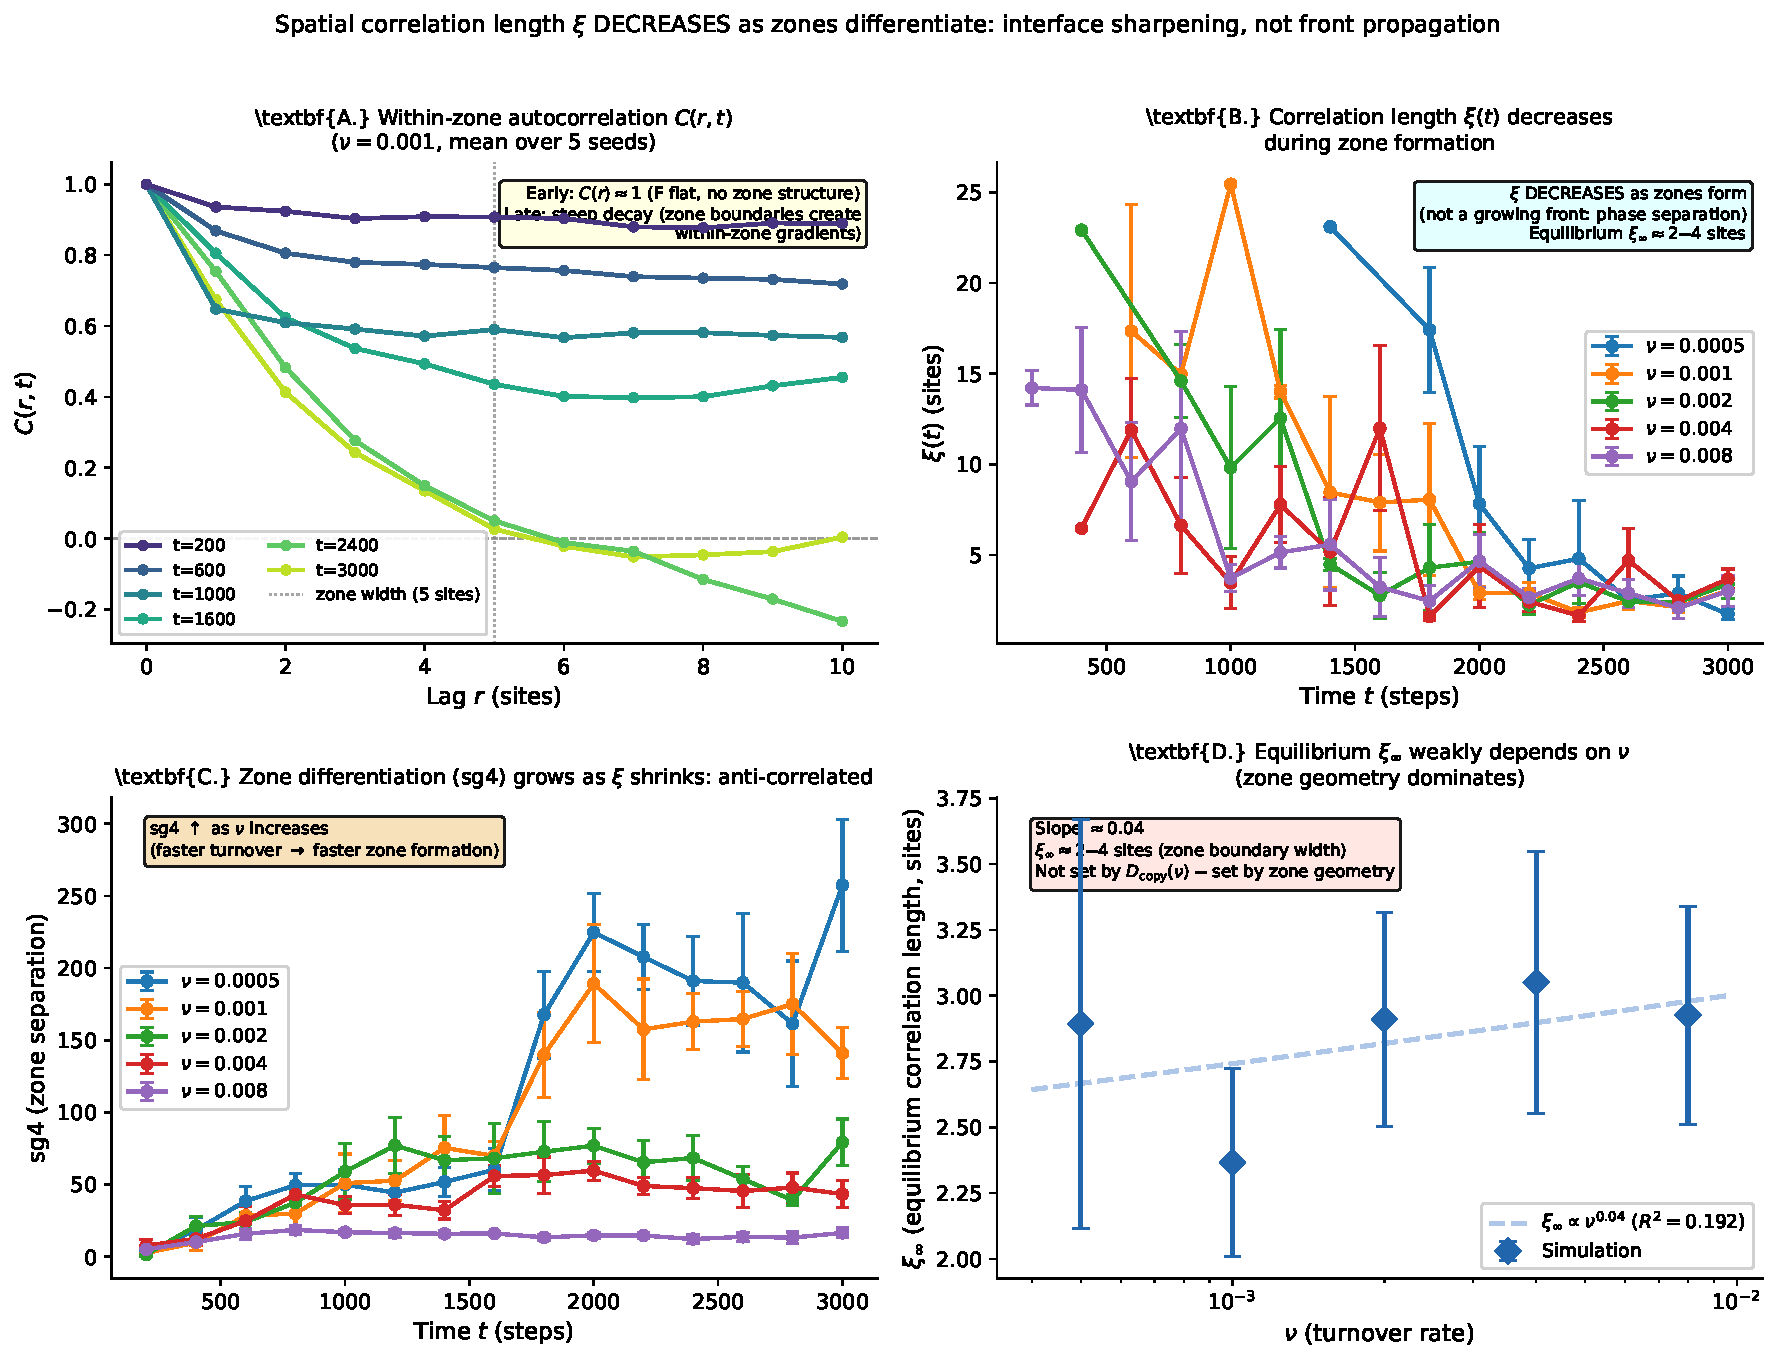
\includegraphics[width=\textwidth]{paper22_figure1.pdf}
\caption{\textbf{Spatial correlation signature of zone formation.}
\textbf{A}: Mean $C(r,t)$ for $\nu=0.001$ at six time points.
Early: $C(r)\approx 1$ (F nearly zero, trivially flat within zones).
Late: steep decay with $\xi_\infty \approx 2$--$3$ sites (zone boundaries create
within-zone gradients).
\textbf{B}: $\xi(t)$ for all $\nu$ values (mean across seeds, outliers $\xi>30$ excluded).
$\xi$ \emph{decreases} monotonically as zone formation proceeds.
\textbf{C}: sg4$(t)$ for all $\nu$ values (note: sg4 \emph{increases} as $\xi$ decreases,
confirming the anti-correlation).
\textbf{D}: Equilibrium $\xi_\infty$ (mean of $t=2400$--$3000$) vs.\ $\nu$.
Nearly flat ($\xi_\infty \propto \nu^{0.04}$, $R^2=0.19$): $\xi_\infty$ is
independent of $\nu$ and set by zone geometry.}
\label{fig:main}
\end{figure}

\end{document}
